\documentclass{article}


\usepackage{arxiv}

\usepackage[utf8]{inputenc} % allow utf-8 input
\usepackage[T1]{fontenc}    % use 8-bit T1 fonts
\usepackage{hyperref}       % hyperlinks
\usepackage{url}            % simple URL typesetting
\usepackage{booktabs}       % professional-quality tables
\usepackage{amsfonts}       % blackboard math symbols
\usepackage{nicefrac}       % compact symbols for 1/2, etc.
\usepackage{microtype}      % microtypography
\usepackage{graphicx}       % define the path of figures
\graphicspath{ {./img/} }
\usepackage{setspace}       % set the space between lines
\doublespacing
\usepackage{subcaption}

\title{State of Public and Private Blockchains:\\Myths and Reality}


\author{
  Matteo Azzarelli\\
  Department of Computer Science\\
  Hong Kong Baptist University\\
  \texttt{18432468@life.hkbu.edu.hk} \\
}

\begin{document}
\maketitle

\begin{abstract}
    In this report we are going to review the main concepts expressed by Dr. C. Mohan in the talk held the day 12 April 2019.
    The main point is introduce the concept of Block Chains (BCs), debunk some myths and discuss about some practically useful private and permissioned BCs.
    Than we will introduce also some details about private BC systems.
\end{abstract}


% keywords can be removed
\keywords{Blockchain}


\section{Introduction}
    First of all we will give you a brief introduction of how they had the idea of blockchain. \cite{wiki-Blockchain} Blockchain is not so recently as the majority part of people think, in fact, the idea was introduced in 1991 by Stuart Haber and W. Scott Stornetta \cite{haber1990time,HistoryBCT}. Their first work involved working on a cryptographically secured chain of blocks whereby no one could tamper with timestamps of documents which is the base of blockchain. Later in 2008, Satoshi Nakamoto released a paper titled "Bitcoin: A Peer-to-Peer Electronic Cash System" \cite{nakamoto2008bitcoin} that signed the real usage of blockchain.
    In fig.\ref{fig:historyOfBlockchain} is showed the progress of blockchain.
    
    \begin{figure}[h]
        \centering
        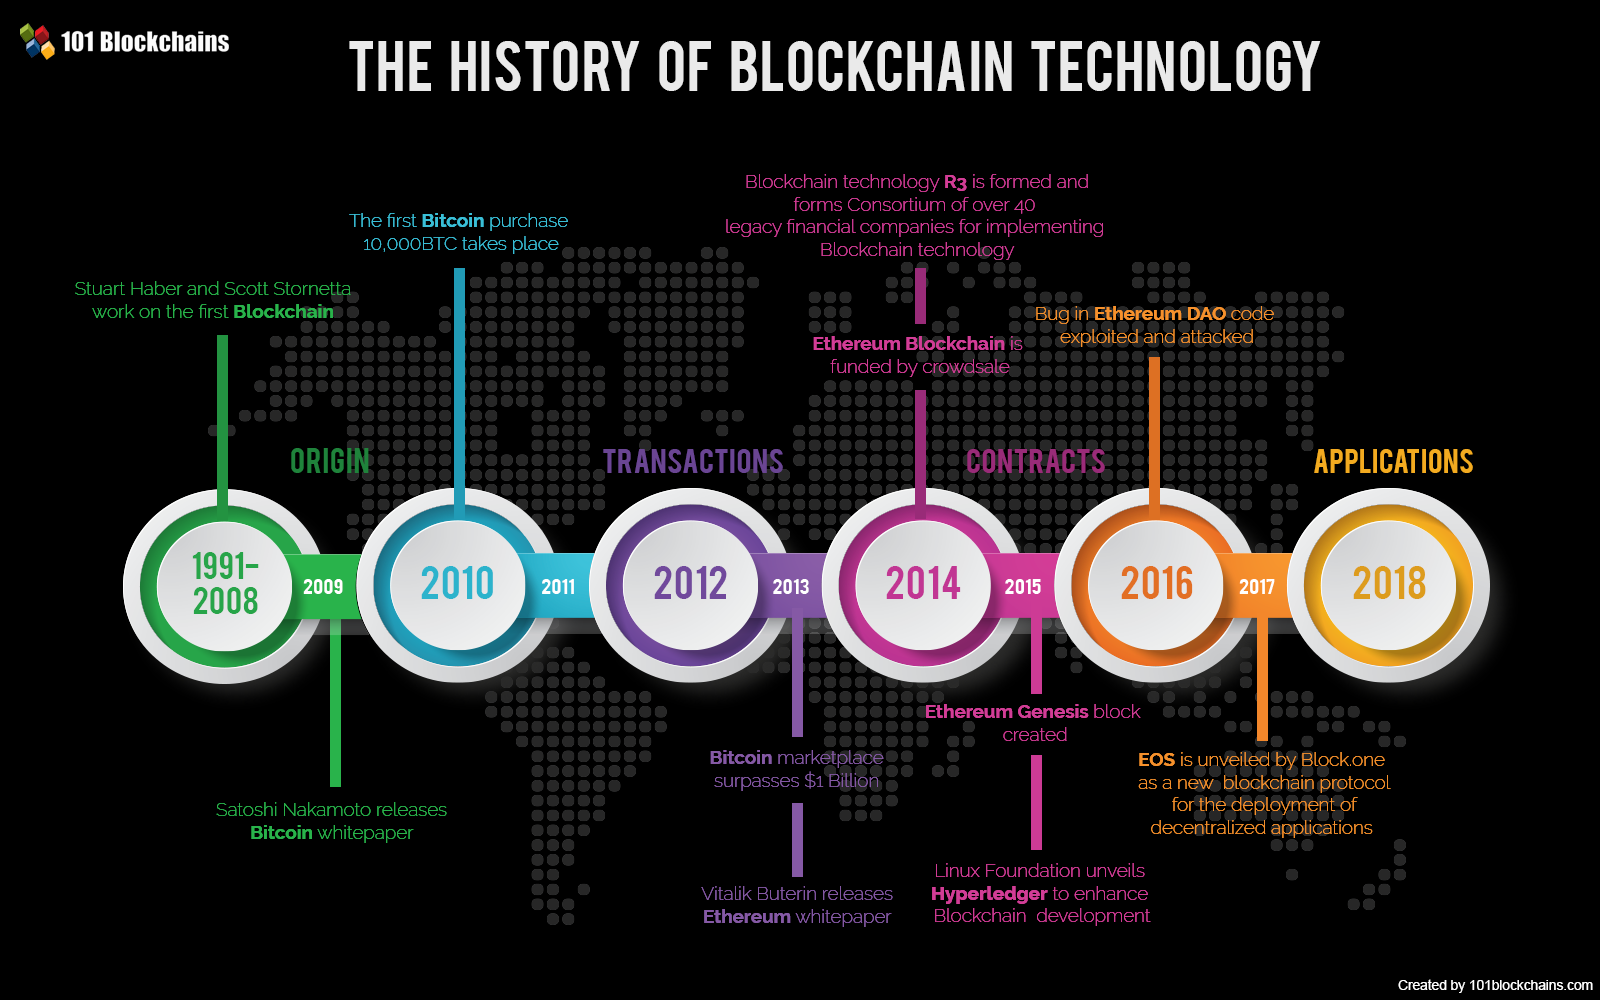
\includegraphics[width=\linewidth]{History_of_Blockchain_Technology.png}
        \caption{Show the main steps of blockchain technology. \cite{HistoryBCT}}
        \label{fig:historyOfBlockchain}
    \end{figure}
    
    At the beginning there was the ledgers, a centralised system where everything were collected and stored, and obviously managed by only one organisation which becomes the 'custodian' and sole manager of the register. So, we have to trust this organisation to manage this records, for instance we have to trust banks to manage our bank accounts.
    
    Subsequently came the decentralised ledgers, which replicated the centralised structure in many smallest nodes. This improve the the degree of robustness and security, but within the field of the trust nothing changed, in fact this is managed by a unique organisation.
    
    Finally the distributed ledgers arrived. The distributed ledgers have eliminated the need for a central element responsible for the functioning and updating of the register.
    
    Blockchain is a specific category of Distributed Ledger Technologies.
    
    There are two fundamental concepts:
    \begin{itemize}
        \item[\textbf{Block}] It is a collection of transaction grouped in a unique block.
        \item[\textbf{Chain}] Each block is strongly connected to the previous one, the last block of the chain include the hash of the previous one. In this way if a block were modified it will broke the chain.
    \end{itemize}
    
    \newpage
    Main different kind of blockchain \cite{wiki-Blockchain, BlockchainPP}:
    \begin{itemize}
        \item \textbf{Public and Permissionless}: The network access is open to anyone and everyone, so it is completely free for everyone that would like to join. The control is distributed and involve every node. Everyone can join and everyone should validate the transaction.
        
        \item \textbf{Private and Permissioned}: The network access and the activity of control and validation are limited to a restricted group of members which follow some guide line (Governance of Blockchain). This kind of blockchain fits applications of companies or organisations that have to guarantee the authentication of participants and of nodes of the blockchain.
        
        
        \item \textbf{Consortium}: It is like the Private, but instead of a single organisation that manage the blockchain, there are more that perform this activity.
        
        \item \textbf{Hybrid}: The network access is limited to group of members that are recognised and authorised. The validation is entrusted to every nodes and all of them contribute to the network security.
    \end{itemize}
    \begin{figure}[h]
        \centering
        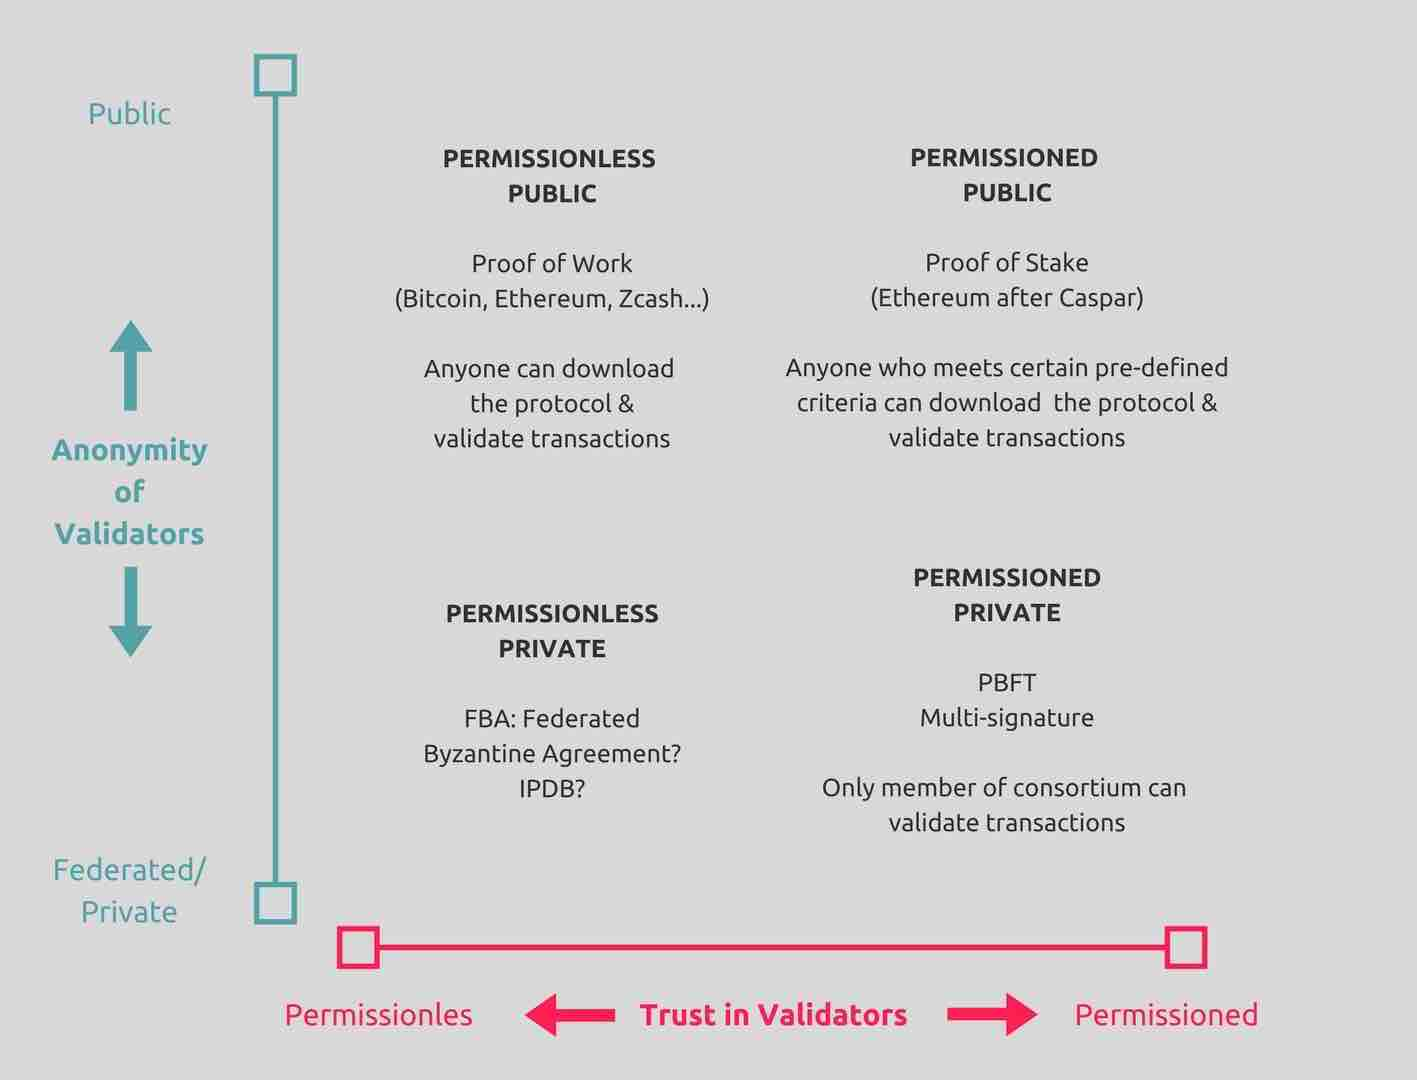
\includegraphics[width=0.8\linewidth]{pppp.jpg}
        \caption{This figure shows the possible combination of public, private and permissionless and permissioned. \cite{fig-pppp}}
        \label{fig:pppp}
    \end{figure}
    
\section{Myth vs reality}
    In this section we are going to discuss some of the common myth regarding blockchain.
    
    First of all, \textbf{Public blockchains are completely decentralized}, this is not really true. For instance, if we consider Bitcoin, this is a public permissionless blockchain, so miners are the entity able to validate transactions.
    
     might seem that if a blockchain is stored on each network node, then special services or authorities cannot stop Bitcoin on a whim, since there is no centralised server or anything like it and there is nobody to turn to if you wanted to close everything.

    In reality, all the "independent" minerals are pooled, in other word they are grouped together under a server in order to combine their computing power. They are based on the assumption that it is better to have a small but stable income than a huge gain perhaps every thousand years and even this is not guaranteed if you are on your own.

    The fig.\ref{fig:bitcoin-mining-pools} shows about 20 of the largest mining pools, but the first 4 control more than 50\% of all the computing power.
    Gaining access to these four control computers alone would give you the chance to double your Bitcoins.
    This, as one can imagine, would devalue Bitcoins somewhat, and doing so is actually quite possible, moreover because most of the pools, as shows in fig.\ref{fig:mining-by-countries}, together with their computing powers, are located within a country, which makes it much easier capture them and gain control over Bitcoins.
    
    
    \begin{figure}[h]
        \begin{minipage}[c]{0.45\linewidth}
            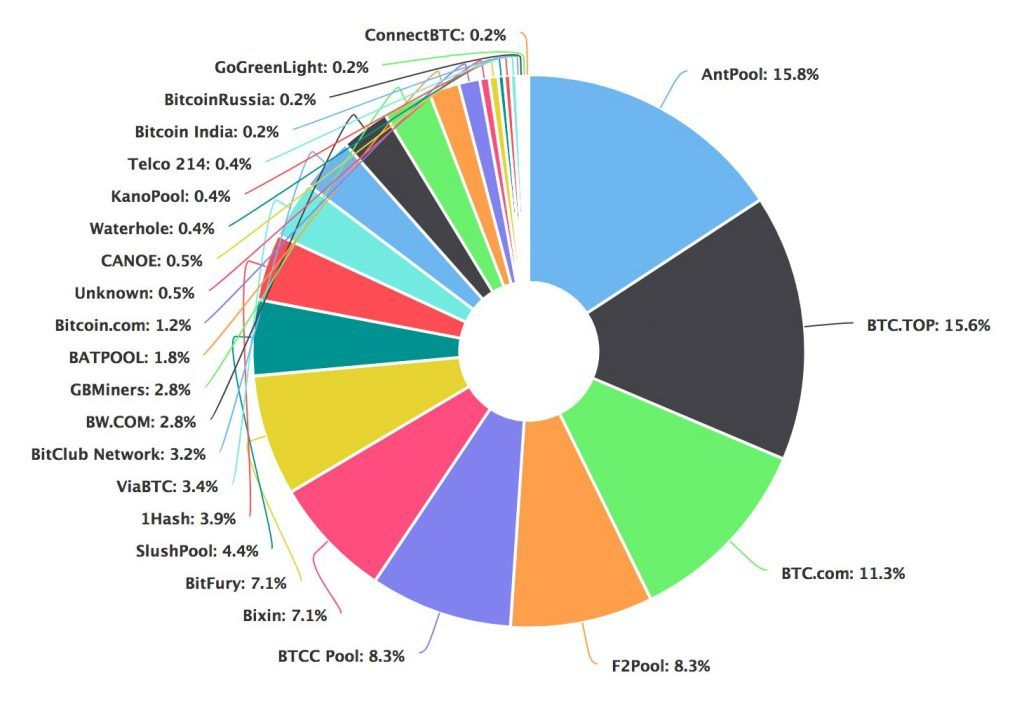
\includegraphics[width=\linewidth]{bitcoin-mining-pools-1024x701.jpg}
            \caption{An estimate of the distribution of computing power among the largest mining pools. \cite{miningpools}}
            \label{fig:bitcoin-mining-pools}
        \end{minipage}
        \hfill
        \begin{minipage}[c]{0.45\linewidth}
            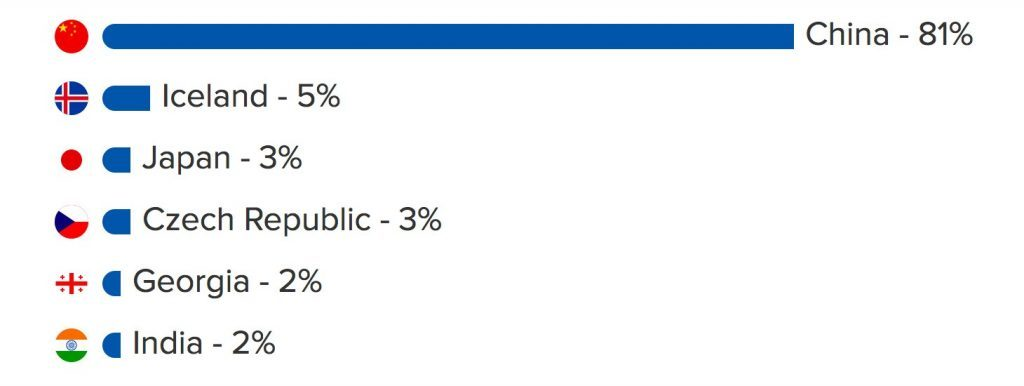
\includegraphics[width=\linewidth]{mining-by-countries-1024x386.jpg}
            \caption{Distribution of mining by country. \cite{miningpools}}
            \label{fig:mining-by-countries}
        \end{minipage}
    \end{figure}
    
\section{Blockchain as a Services - BaaS}
    Now we are going to focus a little more on the Private and Permissioned blockchain.
   
    Blockchain as a Services is a service provided from third parts that offer to their customer the possibility to use cloud base solution in order to build, host and use their own blockchain applications.
    
    The main advantages of these platforms are that they will provide a user friendly environment where the users can build their application without think about how to manages all the necessary tasks and activities to keep the infrastructure agile and operational, and without cover the initial costs of an adequate infrastructure able to supply their requirements.
    
    \begin{figure}[h]
        \centering
        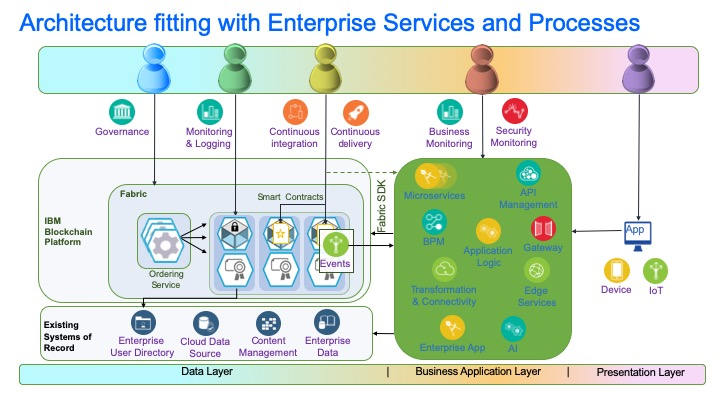
\includegraphics[width=0.8\linewidth]{Slide1.jpeg}
        \caption{Architecture fitting with Enterprise Services and Processes. fig:Architecture (picture from slide of Dr. C. Mohan)}
        \label{fig:fig:Architecture}
    \end{figure}
    
\section{Blockchain Possible Applications}
    Blockchain is not only for financial application, in fact, there are many others sectors that could use this technology, and in particular they could use the BaaS to develop their application.
    
    Now we introduce three of the many possible applications.
    \subsection{Cybersecurity}
        Even if a blockchain register is public, the data communications implemented within it are verified and sent using advanced encryption techniques\cite{cybercecurity}.
        This ensures that the data arrives correctly from the sources to the recipients and that nothing is intercepted in the meantime.
        
        If the blockchain technology were adopted on a larger scale, the likelihood of hacking or attempts to tamper with and intrude on corporate databases could be reduced, due to the fact that the distributed registers are currently considered more robust than many legacy systems. 
        
    \subsection{Academic World}
        The Holbertson School of Software Engineering, based in San Francisco, California, has announced its intention to use blockchain technology to authenticate academic titles and certificates\cite{Holberton}.
        This will ensure that students who claim to have passed the courses of their study program are not able to claim credits that they have not legitimately earned.
        
        Other universities,as it is possible see on this \cite{unic}, have also begun implementing tools based on distributed register technology to ensure greater transparency in the management of academic certificates and in the transcription of degrees and diplomas.
        
        This is why frauds affecting this type of application could be more easily fought, not to mention the savings in terms of time and costs linked to the possibility of avoiding manual checks of thousands of paper documents every year.
        
    \subsection{"Political" elections}
        The elections require the authentication of the identity of the voters, the safe keeping of the registers and an absolutely transparent counting and counting activity to determine the winner. Blockchains can serve as a useful tool for the selection, monitoring and counting of votes in a mirrored manner, clearing the field of any probable attempt at electoral fraud or loss of data and votes. By integrating the selection of votes expressed as operations within the blockchains, voters can be reassured about the correctness and transparency of the final counting of the voting operations, because they are able to directly count the votes themselves and, thanks to the traceability guaranteed by the distributed blockchain databases, they can also be reassured about the fact that the votes have not been modified and that no legitimately expressed votes have been added or, on the contrary, canceled. Follow My Vote has already been used in testing during the last US presidential election as a verifiable end-to-end online voting system. \cite{followmyvote}
        
        Obviously this method could be extended and it is valid for every kind of election.

\bibliographystyle{IEEEtran}  
\bibliography{references}

\end{document}
